\section{目次}
 \begin{itemize}
  \item 対称行列
 \end{itemize}

 \section{対称行列}
 wikiを地道に解読します。\\
 線形代数学における対称行列は、自身の転置行列と一致するような正方行列を言う。
 記号で書けば、行列Aは
 \begin{eqnarray}
  A = A^T
 \end{eqnarray}
 を満たすときの対象であるという。相等しい行列の型は相等しいから、この式を満すのは正方行列に限られる。

 定義により、対称行列の成分は主対角線に関して対象である。すなわち、成分に関して行列$A=(a_{ij})$は任意の添字に関して$a_{ij} = a_{ji}$を満たす。例えば、次の$3 \times 3$行列

 \begin{eqnarray}
  \left(
   \begin{matrix}
	1&7&3\\
	7&4&-5\\
	3&-5&6
   \end{matrix}
   \right)
 \end{eqnarray}
は対象である。任意の正方対角行列は、その非対称対角成分が0であるから、対象である。


\subsection{対角行列って?}
非対角成分が0である行列。\\

同様に、歪対称行列(わいたいしょうぎょうれつ)の対角成分は、自身の転置行列が自身の-1倍となるものをいう。
 \begin{eqnarray}
  A^T = -A
 \end{eqnarray}


\newpage
\chapter{図形の問題}
\section{問題}
\begin{figure}[htbp]
\begin{center}
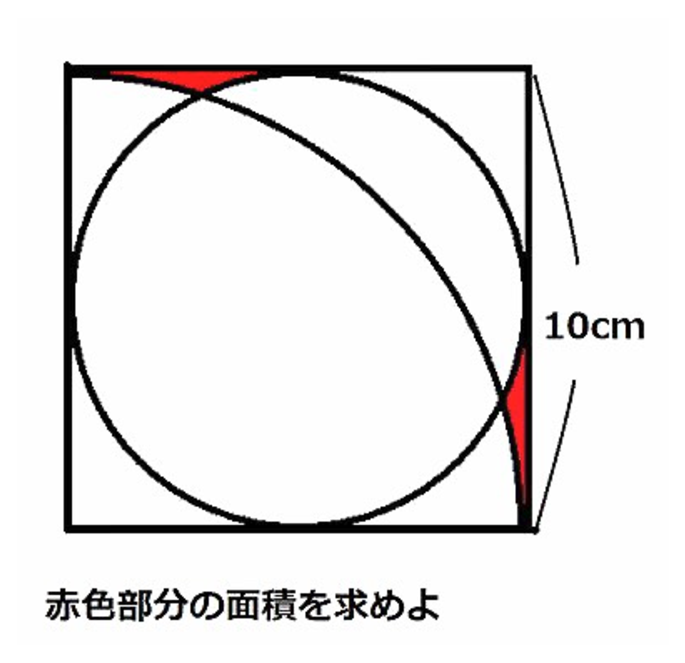
\includegraphics[width=9cm]{../data/1.eps}
\end{center}
\caption{問題図}
\end{figure}

\subsection{解答}
この問題を解く上の方針は、どのように補助線を入れて、どのような方程式を立てるかであるが、ここでは相似な図形を見つけて、それについての方程式を立てる解放を紹介する。
まず、次の図のように補助線を入れて、それぞれの領域に番号をつける。

\newpage
\begin{figure}[htbp]
\begin{center}
\includegraphics[width=9cm]{../data/2.eps}
\end{center}
\caption{領域分割・ネーミング}
\end{figure}


\begin{figure}[]
\begin{center}
\includegraphics[width=6cm]{../data/3.eps}
\end{center}
\caption{相似な図形の抽出}
\end{figure}

\newpage
相似な図形の組み合わせは、上の図のようになる。
緑色領域の相似の関係を用いて、
\begin{eqnarray}
4 \left( \textcircled{1} + \textcircled{2} \right) = 2 \textcircled{1} + \textcircled{2} + \textcircled{3} + \textcircled{4}
\end{eqnarray}

相似な図形の組み合わせは、上の図のようになる。
赤色領域の相似の関係を用いて、
\begin{eqnarray}
4 \left( 2 \textcircled{1} + \textcircled{2} \right)= 4 \textcircled{1}+ \textcircled{2} + \textcircled{3} +2 \textcircled{4} = 100 - 25 \pi
\end{eqnarray}

以上の式より、
\begin{eqnarray}
2 \textcircled{1} &=& \textcircled{4}\\
3 \textcircled{2} &=& \textcircled{3} = 75 - \frac{75}{4} \pi -6 \textcircled{1}
\end{eqnarray}

図形から計算できる領域について、方程式を立てる
\begin{eqnarray}
\textcircled{5} + 4 \left( \textcircled{3} + \textcircled{4} \right) &=& 100\\
\textcircled{5} + 2 \left( \textcircled{2} + \textcircled{3} \right) &=& 50 \pi - 100
\end{eqnarray}
